%\documentclass[mathserif]{beamer}
\documentclass[handout]{beamer}
%\usetheme{Goettingen}
\usetheme{Warsaw}
%\usetheme{Singapore}
%\usetheme{Frankfurt}
%\usetheme{Copenhagen}
%\usetheme{Szeged}
%\usetheme{Montpellier}
%\usetheme{CambridgeUS}
%\usecolortheme{}
%\setbeamercovered{transparent}
\usepackage[english, activeacute]{babel}
\usepackage[utf8]{inputenc}
\usepackage{amsmath, amssymb}
\usepackage{dsfont}
\usepackage{graphics}
\usepackage{cases}
\usepackage{graphicx}
\usepackage{pgf}
\usepackage{epsfig}
\usepackage{amssymb}
\usepackage{multirow}	
\usepackage{amstext}
\usepackage[ruled,vlined,lined]{algorithm2e}
\usepackage{amsmath}
\usepackage{epic}
\usepackage{epsfig}
\usepackage{fontenc}
\usepackage{framed,color}
\usepackage{palatino, url, multicol}
\usepackage{listings}
%\algsetup{indent=2em}


\vspace{-0.5cm}
\title{Generalized and Multilevel Linear Models}
\vspace{-0.5cm}
\author[Felipe Bravo Márquez]{\footnotesize
%\author{\footnotesize  
 \textcolor[rgb]{0.00,0.00,1.00}{Felipe José Bravo Márquez}} 
\date{ \today }




\begin{document}
\begin{frame}
\titlepage


\end{frame}


%%%%%%%%%%%%%%%%%%%%%%%%%%%


\begin{frame}{Generalized and Multilevel Linear Models}
\scriptsize{
\begin{itemize}
\item In this class we will learn two powerful extensions to the linear model, which we have discussed extensively throughout this course.

\item The first extensions is the \textbf{Generalized Linear Model} (GLM) which allows the use of distributions other than Gaussian in the outcome variable.

\item GLMs can be particularly useful when our outcome variable  is binary or bounded to positive values.

\item \textbf{Multilevel models} (also known as hierarchical or mixed effects models), on the other hand, are useful when there are predictors at different level of variation.

\item For example, when studying student performance, we may have information at different levels:  individual students  (e.g., family background), class-level information (e.g., teacher), and school-level information (e.g., neighborhood) \cite{gelman2013bayesian}.


\item Multilevel models extend linear regression to include categorical input variable representing these levels, while allowing intercepts and possibly slopes to vary by level \cite{gelman2006data}.



\end{itemize}



}

\end{frame}


\begin{frame}{Generalized Linear Models}
\scriptsize{
\begin{itemize}
\item The linear regression models of previous classes worked by first assuming a Gaussian distribution over outcomes.
\item Then, we replaced the parameter that defines the mean of that distribution, $\mu$, with a linear model.
\item This resulted in likelihood definitions of the sort:

 \vspace{0.3cm}
 \begin{table}
 \centering
 \begin{tabular}{lr}
$y_i \sim N(\mu_i,\sigma)$ & [likelihood] \\
$\mu_i = \beta_0 + \beta_1 x_i$ & [linear model] \\
\end{tabular}
\end{table}
 \vspace{0.3cm}

\item When the outcome variable is either discrete or bounded, a Gaussian likelihood is not the most powerful choice.

\item Consider for example a count outcome, such as the number of blue marbles pulled from a bag.
\item Such a variable is constrained to be zero or a positive integer.

 
\end{itemize}



} 

\end{frame}

\begin{frame}{Generalized Linear Models}
\scriptsize{
\begin{itemize}


\item The problem of using a Gaussian model with such a variable is that the model wouldn't know that counts can't be negative.

\item So it would happily predict negative values, whenever the mean count is close to zero \cite{mcelreath2020statistical}.

\item In linear regression we basically replace the parameter describing the shape of the Gaussian likelihood $\mu$ with a linear model.

\item The the essence of a Generalized Linear Model (GLM) is to generalize this strategy to probability distributions other than the Gaussian.

\item And it results in models that look like this:

 \vspace{0.3cm}
 \begin{table}
 \centering
 \begin{tabular}{lr}
$y_i \sim \text{Binomial}(n,p_i)$ & [likelihood] \\
$f(p_i) = \beta_0 + \beta_1 x_i$ & [generalized linear model] \\
\end{tabular}
\end{table}
 \vspace{0.3cm}


\end{itemize}



}

\end{frame}


\begin{frame}{Generalized Linear Models}
\scriptsize{
\begin{itemize}


\item  The first change we can note is that likelihood is binomial instead of Gaussian.
\item For a count outcome $y$ for which each observation arises from $n$ trials and with constant expected value $n*p$, the binomial distribution is the de facto choice.

\item The function $f$ represents a \textbf{link} function, to be determined separately from the choice of distribution.

\item Generalized linear models need a link function, because rarely is there a ``$\mu$'', a parameter describing the average outcome.
\item Parameters are also rarely unbounded in both directions, like $\mu$.
\item For example, the shape of the binomial distribution is determined, like the Gaussian, by two parameters.
\end{itemize}



}

\end{frame}


\begin{frame}{Generalized Linear Models}
\scriptsize{
\begin{itemize}

\item But unlike the Gaussian, neither of these parameters is the mean.
\item Instead, the mean outcome is $n*p$, which is a function of both parameters.
\item Since $n$ is usually known (but not always), it is most common to attach a linear model to the unknown part, $p$.
\item But $p$ is a probability, so $p_i$ must lie between zero and one.
\item But there's nothing to stop the linear model $\beta_0 + \beta_1 x_i$ from falling below zero or exceeding one.
\item The \textbf{link} function $f$ provides a solution to this common problem.

\item The link function that is commonly used when working with binomial GLMs is the logit function.

\item It maps a parameter that is defined as a probability $p$ (i.e., $0\leq p\leq 1$), onto a linear model that can take on any real value.

 \vspace{0.3cm}
 \begin{table}
 \centering
 \begin{tabular}{l}
logit$(p_i) = \beta_0 + \beta_1 x_i$ \\ \\
logit$(p_i) = \log\left(\frac{p_i}{1-p_i}\right)$
\end{tabular}
\end{table}
 \vspace{0.3cm}


\end{itemize}



}

\end{frame}


\begin{frame}{Generalized Linear Models}
\scriptsize{
\begin{itemize}

\item If we solve the logit equation for $p_i$ we get:

\begin{equation}
 p_i = \frac{\exp (\beta_0 + \beta_1 x_i)}{1+\exp (\beta_0 + \beta_1 x_i)}
\end{equation}

which is known as the \textbf{sigmoid} function.

\item It is also called the \textbf{logistic} or the \textbf{inverse-logit} function.

\begin{figure}[h!]
	\centering
	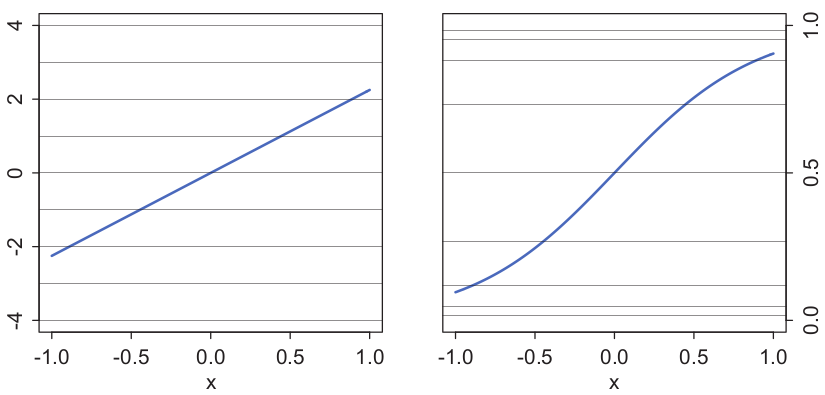
\includegraphics[scale=0.4]{pics/sigmoid.png}
\end{figure}

The logit link transforms a linear model (left) into a probability
(right).

\end{itemize}


}

\end{frame}


\begin{frame}{Generalized Linear Models}
\scriptsize{
\begin{itemize}

\item There are two common flavors of GLM that use binomial likelihood functions and logit link functions:

\begin{enumerate}\scriptsize{
 \item \textbf{Logistic regression}: when the data are organized into single-trial cases $(n=1)$, such that the outcome variable can only take values 0 and 1. In this case the likelihood function can also be represented with a Bernoulli distribution.
\item \textbf{Aggregated binomial regression}: when the outcome can take the value zero or any positive integer up to $n$, the number of trials.}
\end{enumerate}

\item Other distributions that can be used in GLMs are the Exponential, the Poisson and the Gamma distribution.

\item These distributions along with the Gaussian and Binomial are part of the exponential family, which is a set of probability distributions that share some common algebraic properties.

\item We won't go into details of the exponential family here.

\item A very instructive description is given in \cite{ng2012cs229}.

\end{itemize}


}

\end{frame}


\begin{frame}{Expontential Family}
\scriptsize{

\begin{figure}[h!]
	\centering
	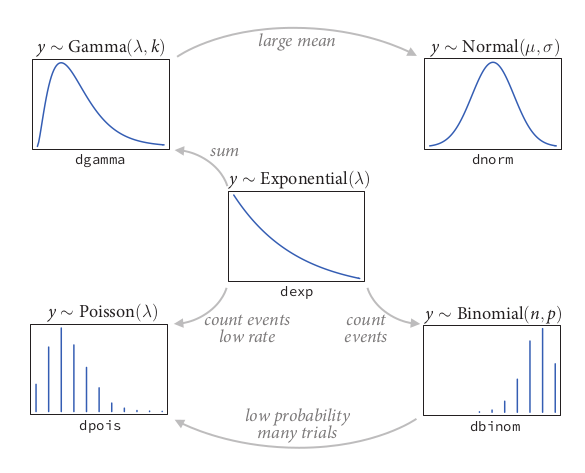
\includegraphics[scale=0.45]{pics/expfamily.png}
\end{figure}
source: \cite{mcelreath2020statistical}

}

\end{frame}


\begin{frame}{Logistic regression: Prosocial chimpanzees.}
\scriptsize{
\begin{itemize}

\item Now we will go through an example of logistic regression given in \cite{mcelreath2020statistical}.

\item The data for this example come from an experiment aimed at evaluating the \textbf{prosocial} tendencies of chimpanzees \cite{silk2005chimpanzees}.

\item A \textbf{focal} chimpanzee sits at one end of a long table with two levers, one on the left and one on the right.


\begin{figure}[h!]
	\centering
	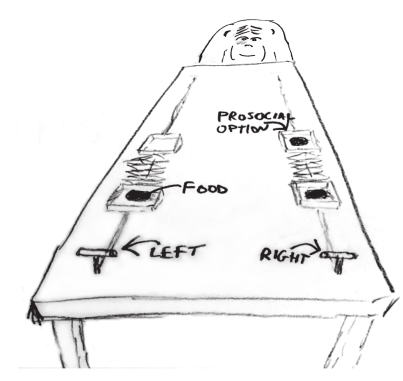
\includegraphics[scale=0.38]{pics/prosocial.png}
\end{figure}


\end{itemize}


}

\end{frame}

\begin{frame}{Logistic regression: Prosocial chimpanzees.}
\scriptsize{
\begin{itemize}

\item On the table are four dishes which may contain desirable food items.
\item The two dishes on the right side of the table are attached by a mechanism to the right-hand lever.
\item The two dishes on the left side are similarly attached to the left-hand lever.
\item When either the left or right lever is pulled by the focal animal, the two dishes on the same side slide towards opposite ends of the table.
\item This delivers whatever is in those dishes to the opposite ends.
\item In all experimental trials, both dishes on the focal animal's side contain
food items.
\item But only one of the dishes on the other side of the table contains a food item.
\item Therefore while both levers deliver food to the focal animal, only one of the levers delivers food to the other side of the table.

\end{itemize}


}

\end{frame}


\begin{frame}{Logistic regression: Prosocial chimpanzees.}
\scriptsize{
\begin{itemize}

\item There are two experimental conditions.
\item In the \textbf{partner} condition, another chimpanzee is seated at the opposite end of the table, as pictured in the figure.
\item In the \textbf{control} condition, the other side of the table is empty. \item Finally, two \textbf{counterbalancing} treatments alternate which side, left or right, has a food item for the other side of the table.
\item This helps detect any \textbf{handedness} preferences for individual focal animals.

\item When human students participate in an experiment like this, they nearly always choose the lever linked to two pieces of food, the prosocial option, but only when another student sits on the opposite side of the table.
\item The motivating question is whether a focal chimpanzee behaves similarly, choosing the prosocial option more often when another animal is present.


\end{itemize}


}

\end{frame}


\begin{frame}{Conclusions}
\scriptsize{

\begin{itemize}
\item Blabla
\end{itemize}


} 
\end{frame}


%%%%%%%%%%%%%%%%%%%%%%%%%%%
\begin{frame}[allowframebreaks]\scriptsize
\frametitle{References}
\bibliography{bio}
\bibliographystyle{apalike}
%\bibliographystyle{flexbib}
\end{frame}  









%%%%%%%%%%%%%%%%%%%%%%%%%%%

\end{document}
